\chapter{Our Tune for the Underlying Event}

This section focus on our work in order to reproduce a similar tune to CP5 one, this is done to test the ability of \textsc{mcnntunes} of being one valid tool for the tuning of Monte Carlo generator with real data. 

\section{Introduction}

We have performed a different tune for the underlying event using the same distributions, shown in \chapRef{sec:Thedistributionsused} used in CP5 tune.

Just a quick reminder for the \textsc{pythia8} settings used in CP5 and in our tune:


we employed bot the \textsc{mcnntunes} described in the previous chapter.

\section{Per Bin Model results}

The training set we use for the PerBin model is composed from approximately 2000 MC runs. 

\figRef{fig:MinBiasPerBinModelResults} 

\begin{figure}[!ht]
	\centering
	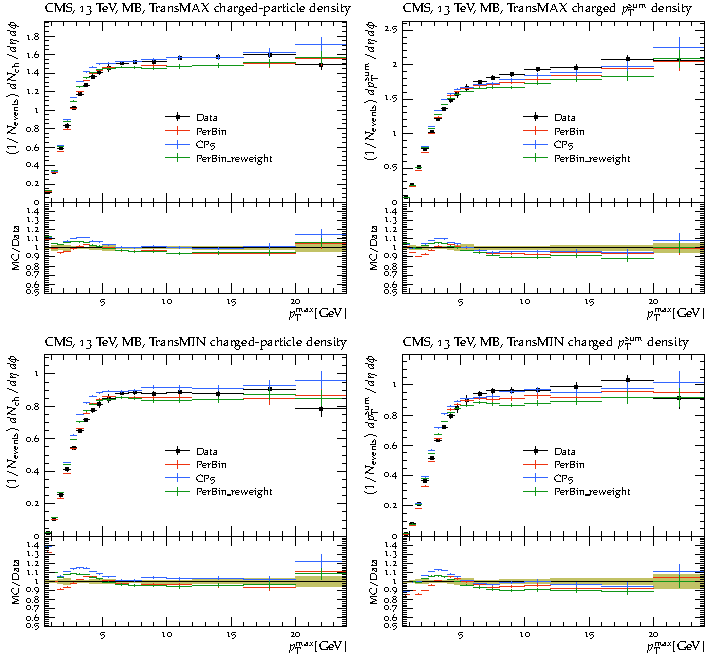
\includegraphics[width=0.8\textwidth]{{img/MinBiasPerBinModelResults1.pdf}}
	\caption{In this figure the data from the $\sqrt{s}=13\ \mathrm{TeV}$ CMS analysis \cite{CMS-PAS-FSQ-15-007} that show the transMAX charged particle density (upper left) and the charged $p_T$-sum density (upper right); the transMIN charged particle density (lower left) and the charged $p_T$-sum density (lower right) as a function of the transverse momentum of the leading charged particle. The CP5 tune is compared to our tune using the PerBin Model. Our tune (red line) is good as the CP5 (blue line) in describing the data. The first bins are the most important they have a smaller experimental error than the higher $p_T$  data. Also the PerBin model with reweight (green line) seems really good in the description of the data. }
	\label{fig:MinBiasPerBinModelResults1}
\end{figure}

\begin{figure}[!ht]
	\centering
	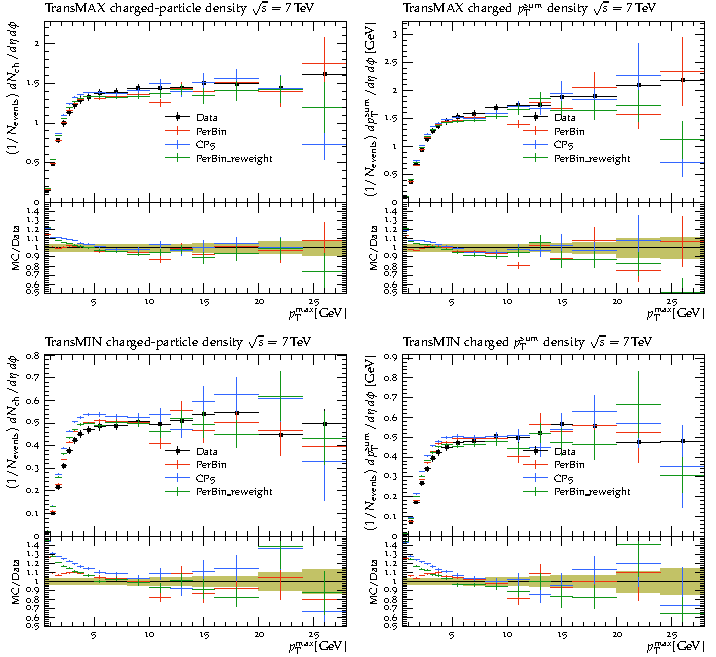
\includegraphics[width=0.8\textwidth]{{img/MinBiasPerBinModelResults4.pdf}}
	\caption{ADD}
	\label{fig:MinBiasPerBinModelResults2}
\end{figure}

\begin{figure}[!ht]
	\centering
	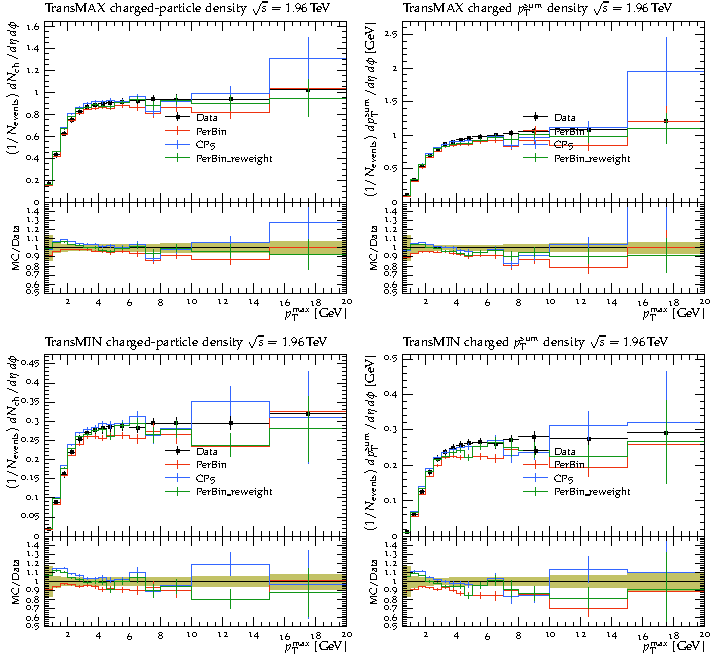
\includegraphics[width=0.8\textwidth]{{img/MinBiasPerBinModelResults5.pdf}}
	\caption{ADD}
	\label{fig:MinBiasPerBinModelResults2}
\end{figure}

\begin{figure}[!ht]
	\centering
	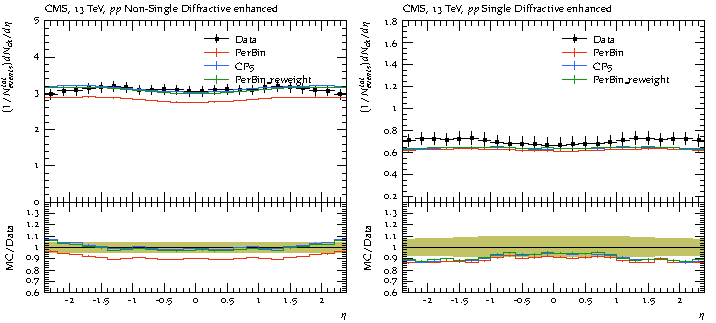
\includegraphics[width=0.8\textwidth]{{img/MinBiasPerBinModelResults2.pdf}}
	\caption{ADD}
	\label{fig:MinBiasPerBinModelResults2}
\end{figure}

\begin{figure}[!ht]
	\centering
	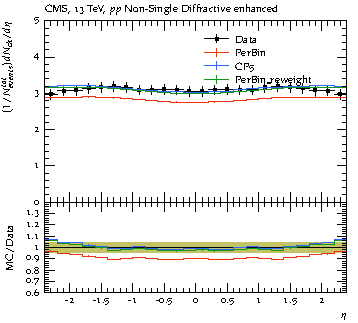
\includegraphics[width=0.42\textwidth]{{img/MinBiasPerBinModelResults3.pdf}}
	\caption{ADD}
	\label{fig:MinBiasPerBinModelResults3}
\end{figure}






